\chapter{Surface Temperature}

Solid surfaces  in CFAST are treated as one-dimensional transient conduction problems. This chapter divides solid surfaces into two major categories -- compartment linings (i.e., walls, ceiling, floor) and targets (i.e., anything that is not a wall, ceiling, or floor). Heat transfer to the inside surface of compartment linings and the front and rear faces (as specified by the user) of targets consists of convection (through the use of empirical correlations) and radiation (calculated by the model using view factors for the fire, gas layers, and compartment surfaces). Heat conduction into a solid surface is calculated via a one-dimensional solution of the heat equation in cartesian or cylindrical coordinates.  The latter is particularly useful for predicting the thermal response of electrical cables.

For compartment linings, the ``outside'' surface is, by default, exposed to the exterior ambient temperature with convection and radiation calculated in a similar manner to the inside surface.  The ``outside'' boundary condition can also be specified as a constant temperature (i.e., the outside surface can be at ambient temperature) or can be connected to the ``outside'' surface of part or all of a second compartment.  For targets, the back surface is simply pointed in a direction opposite that of the front surface with convection and radiation calculated in a similar manner to the front surface.

\section{ Compartment Ceiling, Wall, and Floor Temperature}

In the NIST/NRC and WTC tests, thermocouples and heat flux gauges were positioned at various locations on all four walls of the test compartments, plus on the ceilings and floors. Over the course of 15 experiments, a number of the thermocouples and gauges failed, but because over half of the measurement points were in roughly the same relative location to the fire, the faulty data was discarded based on examining replicate experiments or locations on the opposite wall. Note that Position~8 for the floor and ceiling is not used, simply because the plotting routine is limited to 7 distinct colors and Position~8 is on the opposite side of the compartment to Position~1. Table~\ref{NIST_NRC_Wall_Coords} lists the locations for each test. For each test, eight locations are used for comparison, two on the long (mainly north) wall, two on the short (east) wall, two on the floor, and two on the ceiling.  Of the two locations for each panel, one is considered in the far-field, relatively remote from the fire; one is in the near-field, relatively close to the fire.  How close or far varies from test to test, depending on the availability of working flux gauges. The two short wall locations are equally remote from the fire; thus, one location is in the lower layer, one in the upper.

\begin{table}[p]
\caption[Wall measurement positions for the NIST/NRC series]
{Wall thermocouple and heat flux gauge positions for the NIST/NRC series. The origin of the coordinate system lies on the floor in the southwest
corner of the compartment. The designation ``U'' and ``C'' is irrelevant, and the last digit ``2'' indicates that the thermocouple is measuring the wall temperature rather than the heat flux gauge temperature.}
\begin{center}
\begin{tabular}{|l|c|c|c||l|c|c|c|}
\hline
Name              & $x$   & $y$  & $z$      & Name              & $x$   & $y$   & $z$       \\ \hline \hline
TC North U-1-2    & 3.85  & 7.04 & 1.49     & TC South U-1-2    & 3.86  & 0     & 1.49      \\ \hline
TC North U-2-2    & 3.86  & 7.04 & 3.71     & TC South U-2-2    & 3.86  & 0     & 3.82      \\ \hline
TC North U-3-2    & 9.48  & 7.04 & 1.86     & TC South U-3-2    & 9.54  & 0     & 1.86      \\ \hline
TC North U-4-2    & 12.07 & 7.04 & 1.88     & TC South U-4-2    & 12.08 & 0     & 1.86      \\ \hline
TC North U-5-2    & 17.69 & 7.04 & 1.49     & TC South U-5-2    & 17.69 & 0     & 1.50      \\ \hline
TC North U-6-2    & 17.69 & 7.04 & 3.69     & TC South U-6-2    & 17.74 & 0     & 3.70      \\ \hline \hline
TC East U-1-2     & 21.66 & 1.52 & 1.12     & TC West U-1-2     & 0     & 1.59  & 1.12      \\ \hline
TC East U-2-2     & 21.66 & 1.52 & 2.40     & TC West U-2-2     & 0     & 1.59  & 2.42      \\ \hline
TC East U-3-2     & 21.66 & 5.68 & 1.13     & TC West U-3-2     & 0     & 5.70  & 1.12      \\ \hline
TC East U-4-2     & 21.66 & 5.70 & 2.42     & TC West U-4-2     & 0     & 5.70  & 2.42      \\ \hline \hline
TC Floor U-1-2    & 3.08  & 3.51 & 0        & TC Ceiling U-1-2  & 3.04  & 3.60  & 3.82      \\ \hline
TC Floor U-2-2    & 9.08  & 1.94 & 0        & TC Ceiling C-2-2  & 8.99  & 2.00  & 3.82      \\ \hline
TC Floor U-3-2    & 9.06  & 5.97 & 0        & TC Ceiling C-3-2  & 9.03  & 5.97  & 3.82      \\ \hline
TC Floor U-4-2    & 10.86 & 2.38 & 0        & TC Ceiling C-4-2  & 10.79 & 2.38  & 3.82      \\ \hline
TC Floor C-5-2    & 10.93 & 5.20 & 0        & TC Ceiling C-5-2  & 10.79 & 5.20  & 3.82      \\ \hline
TC Floor U-6-2    & 13.13 & 1.99 & 0        & TC Ceiling C-6-2  & 13.00 & 2.07  & 3.82      \\ \hline
TC Floor U-7-2    & 13.00 & 5.92 & 0        & TC Ceiling C-7-2  & 12.84 & 5.98  & 3.82      \\ \hline
TC Floor U-8-2    & 18.63 & 3.54 & 0        & TC Ceiling U-8-2  & 18.71 & 3.54  & 3.82      \\ \hline
\end{tabular}
\end{center}
\label{NIST_NRC_Wall_Coords}
\end{table}

The WTC test measured ceiling temperatures, both at the surface and beneath a layer of marinite board. Table~\ref{WTC_Ceiling_Coords} below lists the coordinates of the measurement locations relative to the center of the fire pan. Names with ``IN'' appended are measurements made under the marinite board.

\begin{table}[h!]
\caption[Ceiling surface measurement locations for the WTC series]{Locations of ceiling surface temperature measurements relative to the fire pan in the WTC series.}
\begin{center}
\begin{tabular}{|l|c|c|c|}
\hline
Name                & $x$ (m)   & $y$ (m)   & $z$ (m)   \\ \hline \hline
TCC                 & 0.62      & 0.07      & 3.82      \\ \hline
TCN3                & 0.62      & 0.67      & 3.82      \\ \hline
TCS3                & 0.62      & -0.53     & 3.82      \\ \hline
TCE7                & 2.18      & 0.07      & 3.82      \\ \hline
TCW7                & -1.15     & 0.07      & 3.82      \\ \hline \hline
TCCIN               & 0.62      & 0.07      & 3.83      \\ \hline
TCN3IN              & 0.62      & 0.67      & 3.83      \\ \hline
TCS3IN              & 0.62      & -0.53     & 3.83      \\ \hline
TCE4IN              & 1.28      & 0.07      & 3.83      \\ \hline
TCW4IN              & 0.05      & 0.07      & 3.83      \\ \hline
\end{tabular}
\end{center}
\label{WTC_Ceiling_Coords}
\end{table}

Figure \ref{fig:Surface_Temperature_Scatter} shows a comarison of predicted and measured values for total heat flux. Appendix B provides comparisons of heat flux and surface temperature on cable and surface targets.  The following trends are notable comparing CFAST predictions to experimental measurements.
\label{Surface Temperature}
\label{Wall Temperature}
\label{Ceiling Temperature}
\label{Floor Temperature}

\begin{figure}
\begin{center}
\includegraphics[width=4in]{FIGURES/ScatterPlots/Surface_Temperature}
\end{center}
\caption{Comparisons of Measured and Predicted  Compartment Surface Temperature} \label{fig:Surface_Temperature_Scatter}
\end{figure}

\begin{itemize}
\item CFAST predicts compartment surface temperature within \Surfacetempavg ~\%.  Still, there is considerable scatter in the data indicating a higher uncertainty in prediction of surface temperature  like those observed in heat flux and temperature to targets.
\item Typically, CFAST over-predicts the far-field fluxes and temperatures and under-predicts the near-field measurements.  This is understandable, given that any two-zone model predicts an average representative value of gas temperature in the upper and lower regions of a compartment.  Thus, the values predicted by CFAST should be an average of values near the fire and those farther away.
\item However, differences for the ceiling and (particularly) floor temperatures are higher, with a more pronounced difference between the near-field and far-field comparisons.  In addition to the limitations of the two-zone assumption, calculations of the flux to ceiling and floor surfaces are further confounded by the simple point-source calculation of radiation exchange in CFAST for the fire source.  In CFAST, the fire is assumed to be a point source of energy located at  mid-height in the fire rather than a three-dimensional flame surface radiating to surroundings.  With the fire typically at the floor surface, this makes the calculation of flux to the floor surface (and thus floor temperature) inherently less accurate than for other surfaces.
\item CFAST is capable of predicting the surface temperature of a wall, assuming that its composition is fairly uniform and its thermal properties are well-characterized.  Predictions are typically within 10~\% to 30~\%.  Generally, CFAST over-predicts the far-field temperatures, and under-predicts the near-field measurements.  This is consistent with the single representative layer temperature assumed by zone fire models.
\item CFAST predictions of floor temperature are more problematic because of the simple point-source calculation of radiative exchange between the fire and compartment surfaces.
\end{itemize}

\section{Target Temperature}

Target temperature and heat flux data are available from the NIST/NRC test series.  In the NIST/NRC tests, the targets are different types of cables in various configurations: horizontal, vertical, in trays, or free-hanging. Since these tests are intended to represent electrical cables, they are modeled as cylindrical targets. Targets in the SP AST and WTC tests, intended to represent various components of the building structure, are modeled as normal thermally-thick targets in CFAST.

The SP Adiabatic Surface Temperature Experiments included measurements of gas, plate thermometer, and steel temperatures for compartment and pool fire experiments conducted at SP, Sweden. Only the compartment fire experiments are included in the CFAST comparisons. Three additional experiments were conducted at SP, Sweden, in 2011, in which a 6~m long, 20~cm diameter vertical column was positioned in the middle of 1.1~m and 1.9~m diesel and 1.1~m heptane pool fires~\cite{Sjostrom:AST}. Gas, plate, and steel surface temperature measurements were made at heights of 1~m, 2~m, 3~m, 4~m, and 5~m above the pool surface. At heights of 1~m, 3~m, and 5~m, these measurements were made at only one angular position. However, at 2~m and 4~m, the measurements were made at four positions. At these heights, two conventional plates thermometers were positioned approximately 10~cm from the column surface, along with two special plate thermometers (SPT) that were installed flush with the column surface. At each height, comparable predictions were made with CFAST using normal, thermally-thick targets.

The compartment for the WTC experiments contained a hollow box column roughly 0.5~m from the fire pan, two trusses over the top of the pan, and one or two steel bars resting on the lower truss flanges. In Tests 1, 2 and 3, the steel was bare, and in Tests 4, 5 and 6, the steel was coated with various thicknesses of sprayed fire-resistive materials. The column was instrumented near its base (about 0.5~m from the floor, middle (1.5~m), and upper (2.5~m). Four measurements of steel (and insulation) temperatures were made at each location, for each of its four sides. These elements were modeled using thin sheet obstructions with a resolution of 10~cm. In addition to the steel structural elements, five cylinders (``slugs'') of nickel~200 ($\ge$ 99~\% nickel), 25.4~cm long and 10.2~cm in diameter, were positioned 50~cm north of the centerline in the WTC experiments. Slugs 1 through 5 were 2.92~m, 1.82~m, 0.57~m, 0.05~m, and 1.56~m, respectively, from the longitudinal axis of the fire pan. All the slugs were 50~cm north of the lateral axis. The fire pan measured 2~m by 1~m. Four thermocouples were inserted into each slug at various locations. All four temperatures for each slug were virtually indistinguishable.Targets were modeled with normal thermally-thick targets in CFAST.

Figure \ref{fig:Target_Temperature_Scatter} shows a comparison of predicted and measured values for total heat flux. Appendix B provides comparisons of heat flux and surface temperature on cable and surface targets.  The following trends are notable comparing CFAST predictions to experimental measurements.
\label{Target Temperature}

\begin{figure}
\begin{center}
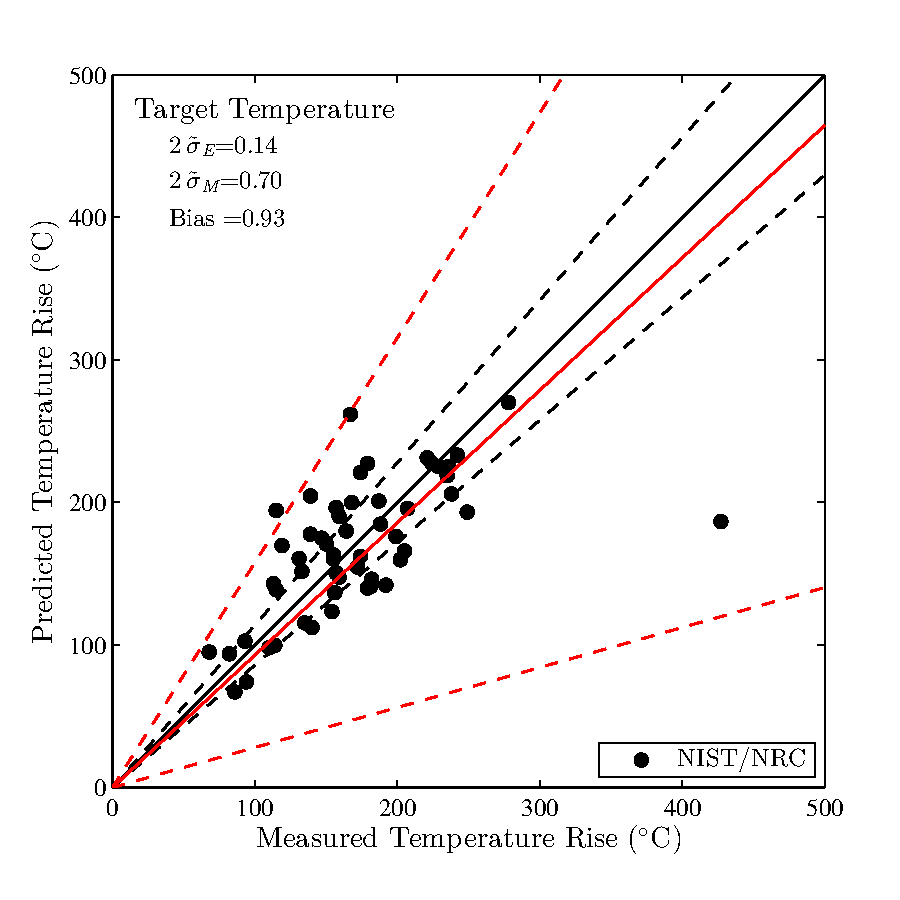
\includegraphics[width=4in]{FIGURES/ScatterPlots/Target_Temperature}
\end{center}
\caption{Comparisons of Measured and Predicted Target Temperature} \label{fig:Target_Temperature_Scatter}
\end{figure}

\begin{itemize}
\item Overall, the comparisons of target temperature show larger relative differences than other quantities. This is to be expected since the target flux and temperature are inherently local quantities.
\item The difference between predicted and measured cable surface temperatures in the NIST/NRC experiments is often within experimental uncertainty, with exceptions.  Target temperature predictions average within \Targtempavg ~\% of experimental values while predictions of cable temperatures average within 2 \% of experimental values.  However, there is considerable spread in the relative differences.  Accurate prediction of the surface temperature of the cable should indicate that the flux to the target (a combination of radiation from the fire, surrounding surfaces, and the gas layers, along with convection from the surrounding gas) should be correspondingly accurate.
\item For both the SP AST and WTC tests, the underlying weakness of a zone model in predicting local temperatures is apparent with clear horizontal banding for both test series.  Since CFAST target temperatures are largely driven by the uniform gas layer temperature predicted by the model, targets at the same height but at different horizontal locations within a compartment will show similar temperatures.  From a validation viewpoint, this increases the uncertainty of the predictions considerably.
\end{itemize}


